% $Id: assembly.tex 8331 2020-11-19 05:17:40Z mskala $

%
% MSK 011 build instructions
% Copyright (C) 2018, 2020  Matthew Skala
%
% This program is free software: you can redistribute it and/or modify
% it under the terms of the GNU General Public License as published by
% the Free Software Foundation, version 3.
%
% This program is distributed in the hope that it will be useful,
% but WITHOUT ANY WARRANTY; without even the implied warranty of
% MERCHANTABILITY or FITNESS FOR A PARTICULAR PURPOSE.  See the
% GNU General Public License for more details.
%
% You should have received a copy of the GNU General Public License
% along with this program.  If not, see <http://www.gnu.org/licenses/>.
%
% Matthew Skala
% https://northcoastsynthesis.com/
% mskala@northcoastsynthesis.com
%

\chapter{Building the module}

The circuit board  has components on both sides, which makes the order of
assembly important; installing the wrong components first may make it
difficult to safely maneuver the soldering iron to install later components
without damaging the already-installed components.

\section{Preliminaries}

Count out the right number of everything according to the bill of materials
on page~\pageref{cha:bom}. 

\noindent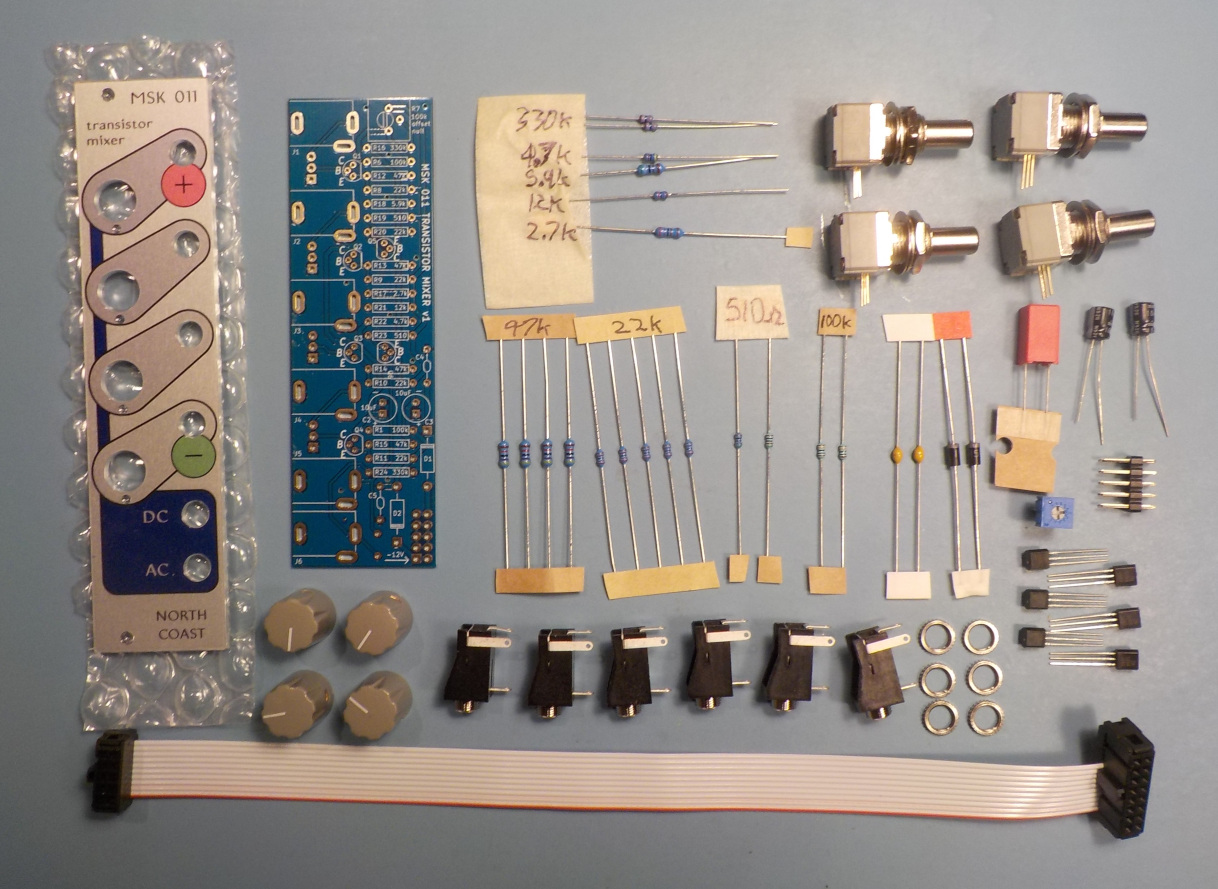
\includegraphics[width=\linewidth]{module-parts.jpg}

\section{Some notes on knobs}

The first batch of knobs I ordered for North Coast products turned out to
have serious quality problems, specifically with the setscrews that hold the
knobs onto the potentiometer shafts.  Some of the screws had marginal
threads that would strip when the screw was tightened, and I ended up having
to do a bunch of extra testing and ship extra knobs to some customers to
replace any that might fail.  Later batches have also had issues, although
they're under better control now because the bad first batch served as a
warning to step up the testing procedures.  Starting with kits prepared in
August 2019, I switched to blue knobs with 100\%\ testing; in September
2020, I switched to a new manufacturer, and knobs that are a slightly darker
shade of blue.  Although all the knobs I ship in kits now have been tested
and passed at least twice, and should be fine to use, I am also shipping
spare setscrews in any kits with knobs from batches where a signficant
number of knobs failed testing.

Here are some things to be aware of as a kit builder.

\begin{itemize}
\item Some photos in these instructions were taken with the older grey
knobs, and some dealers may still have kits containing grey knobs in their
stock, but newer kits will have blue knobs.

\item Do not overtighten the setscrews when attaching the knobs!  The screw
should be tight enough to hold the knob onto the shaft, but there's no
advantage to making it tighter than that, and overtightening may risk
destroying the screw thread or damaging the drive slot.

\item If, despite my efforts to make sure no bad screws get sent to
customers, you still get a bad screw that cannot be tightened and no spare
for it, then please contact me.

\item If you want to source an exact replacement for the setscrew, it should
be an M3$\times$3mm flat-tip slotted setscrew, which is also sometimes
called a ``grub screw,'' made of RoHS-compliant brass (possibly by
exemption).  Stainless steel is fine too, and I may sometimes ship stainless
steel screws instead of brass if I can find a reliable source for them;
plain steel should not be used here for galvanic corrosion reasons. 
Hex-socket screws are fine if you have the driver for them, but I don't ship
those because I'm not sure all DIY builders do have the right driver.

\item Because it's a standard M3 thread, in a pinch it's possible to
substitute a plain M3 machine screw such as are commonly used with Eurorack
cases, although one of those would obviously look less nice.
\end{itemize}

\pagebreak

\section{Panel components}

The components that go through the panel should be installed first because
soldering them may be difficult later.  First, place the six jack sockets J1
to J6 in their locations on the board.  Note that the silkscreen for these
may not be exactly as shown.  I had one batch of boards in which the
silkscreen lines perpendicular to the panel were missing.  The text, and the
short lines showing the backs of the jack bodies, should still make clear
where the jacks go.

\noindent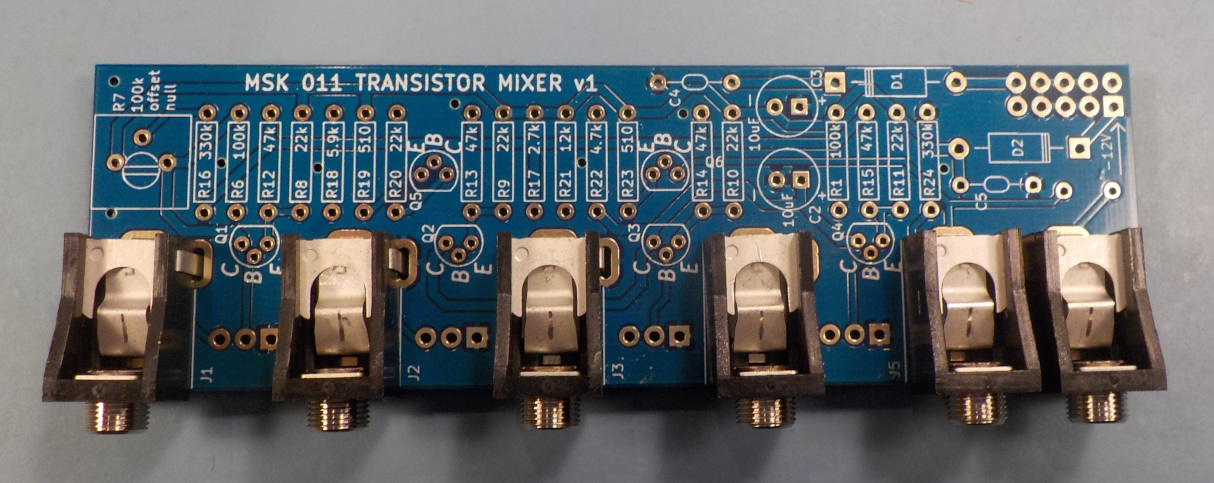
\includegraphics[width=\linewidth]{jacks.jpg}

Attach the panel to the jack sockets using the knurled nuts that came with
the jacks.  It should be snug, but not tight; you will be removing the panel
again soon.

\noindent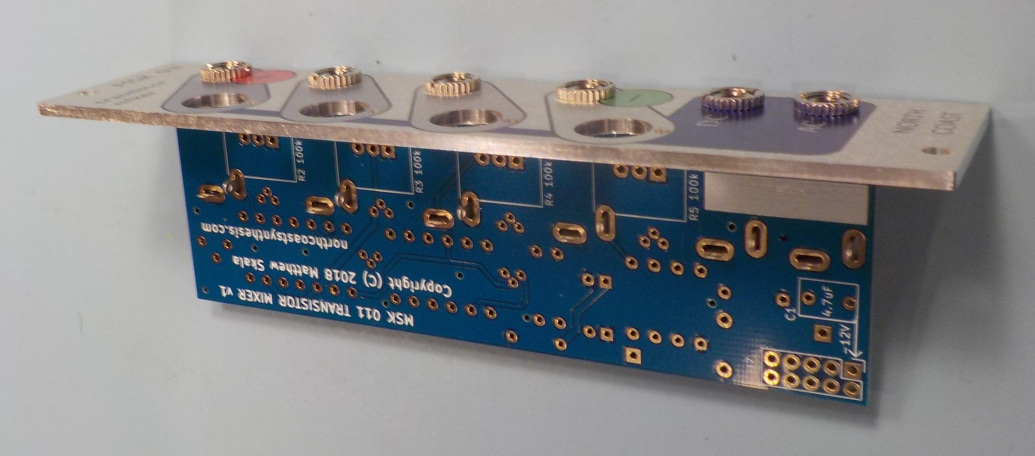
\includegraphics[width=\linewidth]{jacks-panel.jpg}

Solder the jack sockets in place.

Remove the panel, place the four 100k$\Omega$ panel potentiometers R2--R5 in
their locations on the opposite side of the board, then reinstall the panel. 
As with the jack sockets, it is possible that the silkscreen markings for
these on the board may not be exactly as shown in the photo here.
Use just a nut (not the other mounting hardware) to hold the potentiometers
in place, and again tighten them only moderately, because this is a
temporary assembly.  Depending on the board tolerances, the legs of the
potentiometers may be bent somewhat when installed this way.  Be careful
when soldering them not to damage the nearby plastic of the jack sockets. 
Because cleaning these joints may be difficult, it is advisable to use
no-clean and not water-washable solder flux.  Similarly, because of the
limited access it is probably better not to attempt to clip the leads after
soldering.

\noindent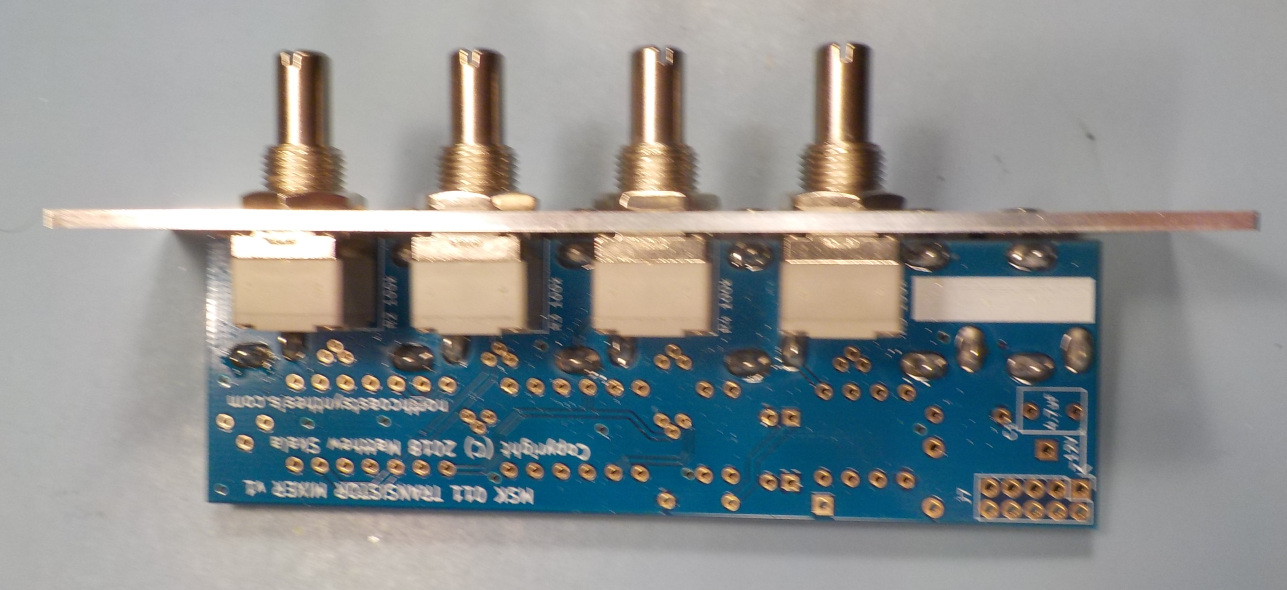
\includegraphics[width=\linewidth]{pots-panel.jpg}

At this stage you have the option to leave the panel attached through the
rest of the assembly, which will protect the pots from getting bent out of
position, or remove it, which will allow for more convenient access to
solder other components.  For the photos in these instructions, I have
removed the panel for a clearer view of the components, but it may really be
a better idea to leave it in place.  Without the panel, the pots are
supported delicately on their legs and may easily be bent or damaged by
careless handling.

Note it is not recommended to try to do the jack sockets and potentiometers
in a single step without removing the panel in between, because of the
difficulty of making the large solder joints on the jacks while the
potentiometers are in place without damaging them.  This assembly routine,
although convoluted, really seems to be the safest and easiest way to do it. 
Having parts on both sides of a single board is part of the price paid for
keeping the module to only 6HP width.

\section{Fixed resistors}

Resistors are never polarized.  I like to install mine in a consistent
direction for cosmetic reasons, but this is electrically unnecessary.  In
this module, metal film 1\%\ resistors are recommended for all fixed-value
resistors.  These will usually have blue bodies and four colour bands
designating the value, plus a fifth band for the tolerance, brown in the
case of 1\%.  These are the resistors normally shipped in the
North Coast kits, but we may occasionally ship better-tolerance resistors (such
as 0.5\%) if we are able to source them at a good price. 
Accordingly, I mention only the four value band colours for this type of
resistor; if you are using resistors with other codes, you are responsible
for knowing them.  Note that colour codes on metal film 1\% resistors are
often ambiguous (reading from one end or the other end may give two
different values, both plausible) and some of the colours are hard to
distinguish anyway.  If in doubt, always measure with an ohmmeter before
soldering.

\pagebreak

Install the two 510$\Omega$ (green-brown-black-black) resistors R19 and R23. 
These are emitter degeneration resistors for the transistors Q5 and Q6; they
make the gain of those amplifying transisters smaller and more controllable.

\nopagebreak
\noindent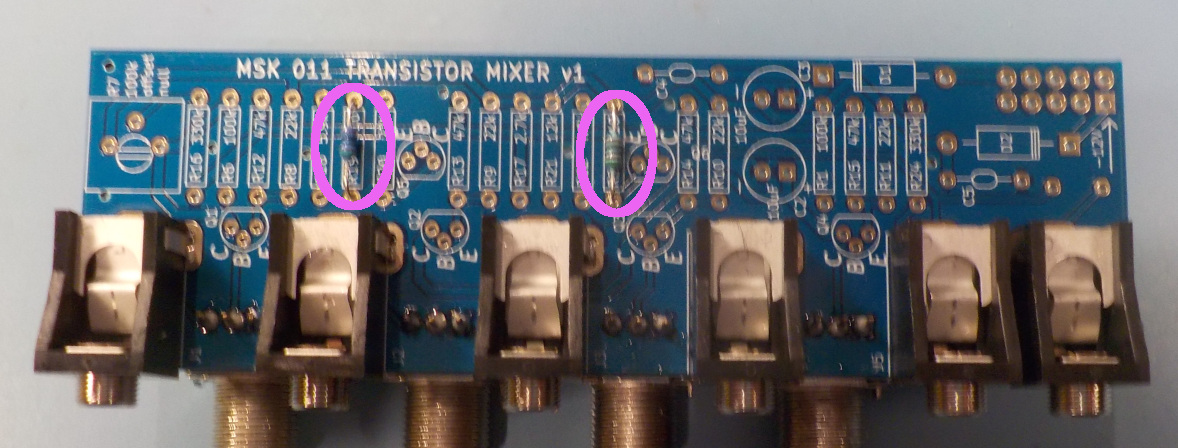
\includegraphics[width=\linewidth]{res-510.jpg}

Install the 2.7k$\Omega$ (red-violet-black-brown) resistor R17.  This
resistor scales the output of the passive mixing network to the appropriate
range for the output amplifier.

\nopagebreak
\noindent\includegraphics[width=\linewidth]{{res-2.7k}.jpg}

Install the 4.7k$\Omega$ (yellow-violet-black-brown) resistor R22.  This
resistor sets the gain for the second stage of the output amplifier.  Do not
confuse it with the 47k$\Omega$ resistors, which have a similar colour code.

\nopagebreak
\noindent\includegraphics[width=\linewidth]{{res-4.7k}.jpg}

Install the 5.9k$\Omega$ (green-white-black-brown) resistor R18.  This
resistor sets the gain for the first stage of the output amplifier.

\nopagebreak
\noindent\includegraphics[width=\linewidth]{{res-5.9k}.jpg}

\pagebreak

Install the 12k$\Omega$ (brown-red-black-red) resistor R21.  This resistor
is part of the network that links the two stages of the output amplifier.

\nopagebreak
\noindent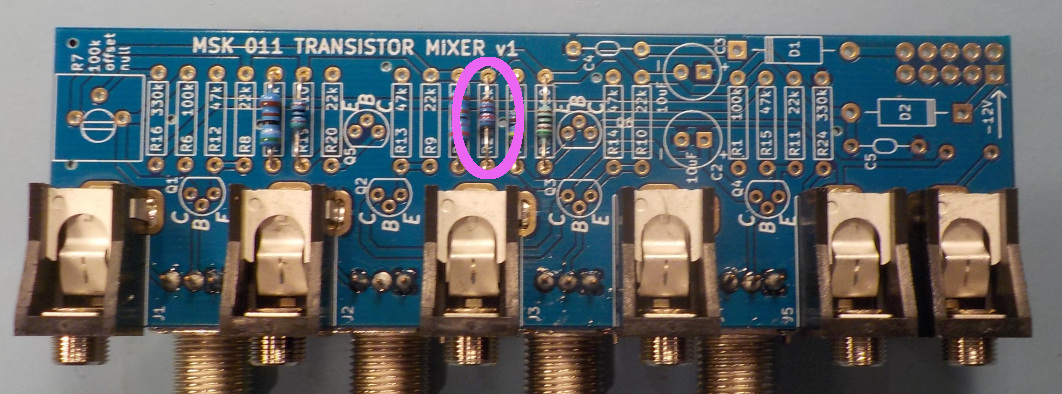
\includegraphics[width=\linewidth]{res-12k.jpg}

Install the four 22k$\Omega$ (red-red-black-red) resistors R8 to R11 and
R20.  Most of these provide voltage pull-down for the input buffers; R22 is
part of the network linking the stages of the output amplifier.

\nopagebreak
\noindent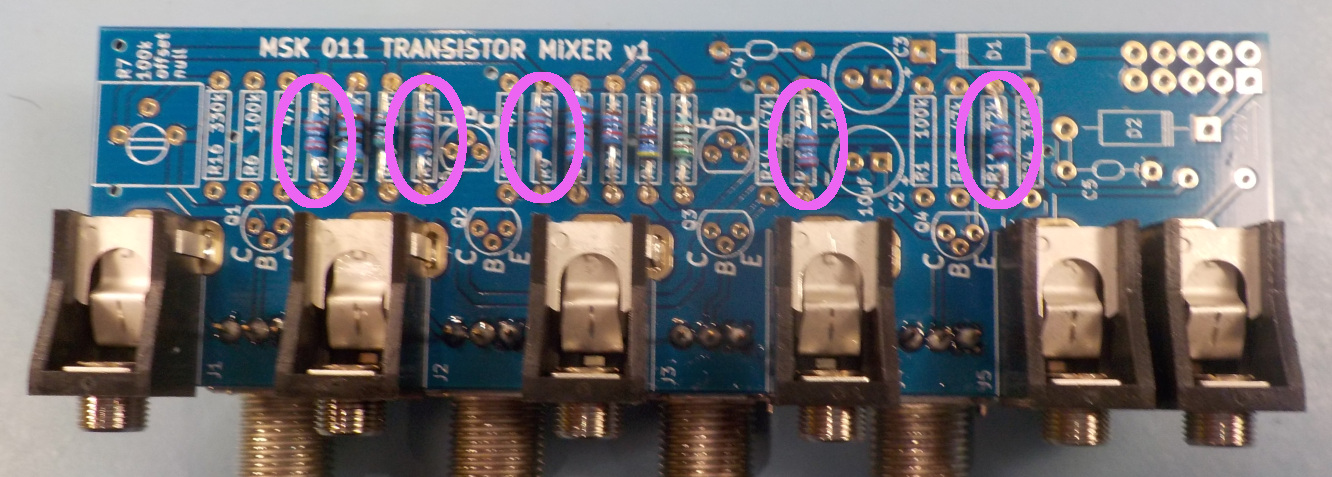
\includegraphics[width=\linewidth]{res-22k.jpg}

Install the four 47k$\Omega$ (yellow-violet-black-red) resistors R12 to R15. 
These resistors form the mixing network between the input buffers and output
amplifier.

\nopagebreak
\noindent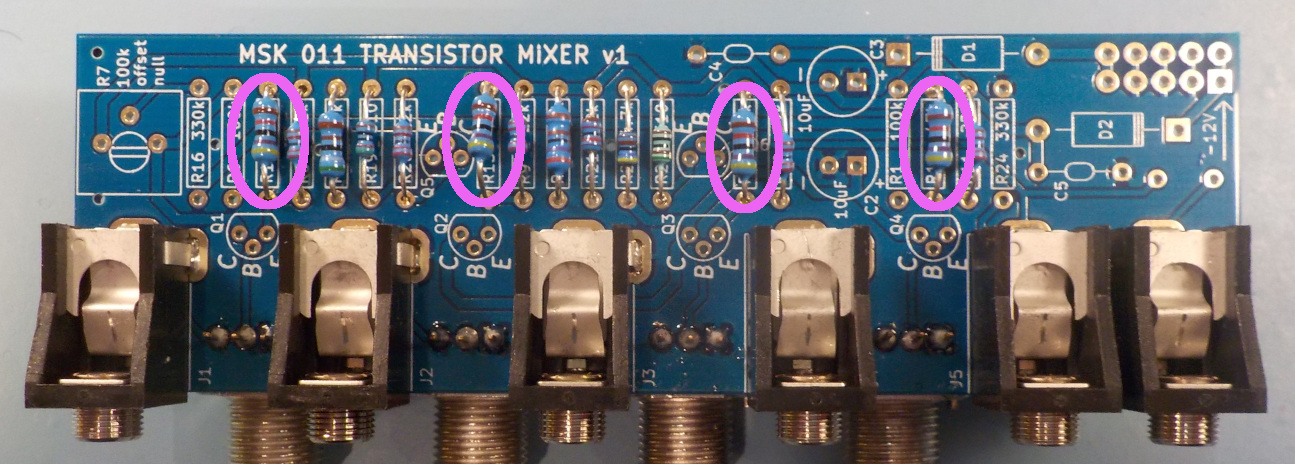
\includegraphics[width=\linewidth]{res-47k.jpg}

Install the two 100k$\Omega$ (brown-black-black-orange) resistors R1 and R6. 
These provide normalling voltages for the top and bottom knobs, to allow
introduction of a DC offset in control voltage mixing.

\nopagebreak
\noindent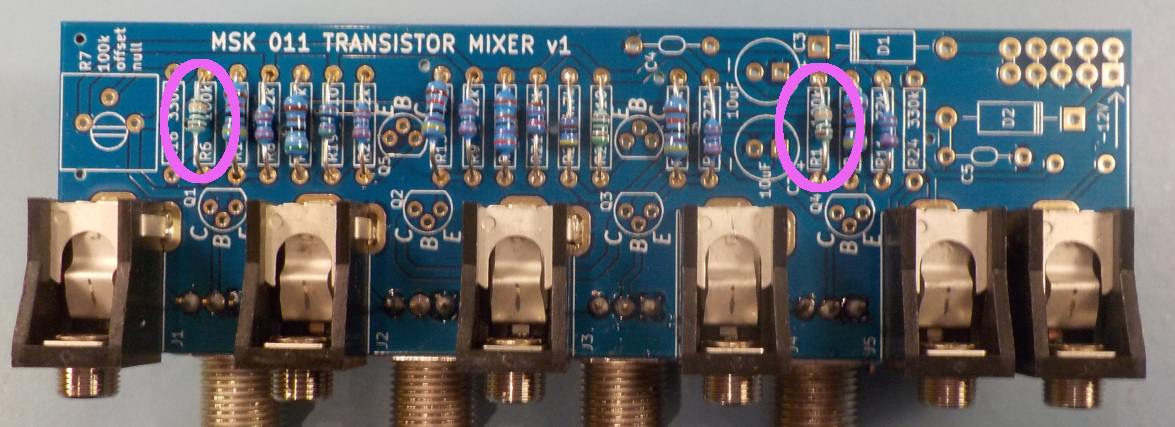
\includegraphics[width=\linewidth]{res-100k.jpg}

\pagebreak

Install the two 330k$\Omega$ (orange-orange-black-orange) resistors R16 and
R24.  R16 controls the scale of the offset null trimmer, and R24 eliminates
DC offset at the AC-coupled output.

\nopagebreak
\noindent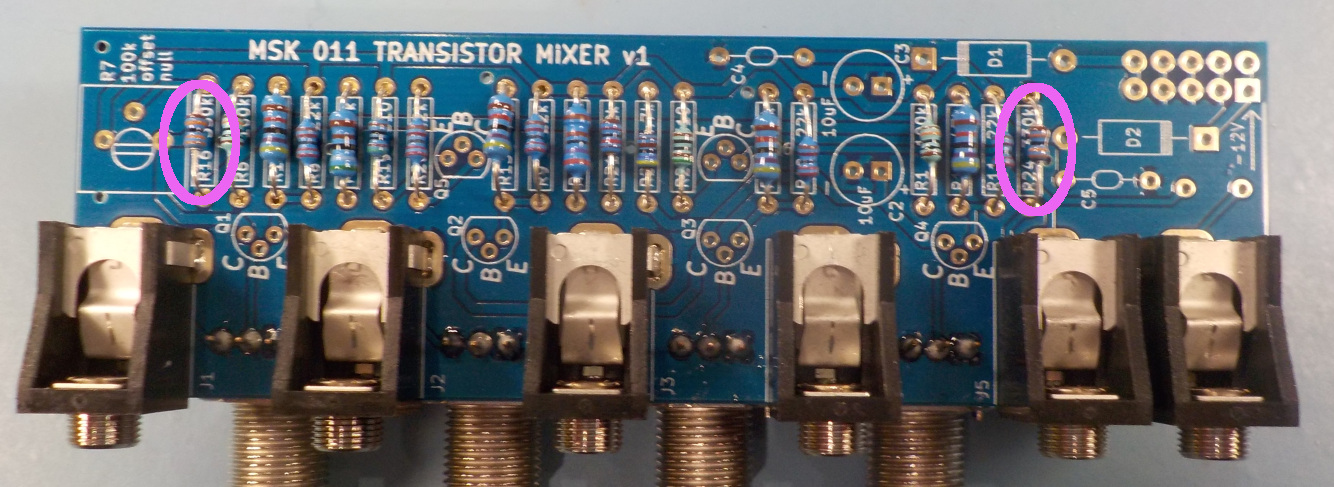
\includegraphics[width=\linewidth]{res-330k.jpg}

\section{Trimmer potentiometer}

Trimmers are not exactly polarized, but the three legs of a trimmer serve
different functions and need to be connected to the right holes.  The
physical arrangement of the legs and corresponding holes should make it
impossible to install the trimmer wrong way round.

Also note that the silkscreened footprint for the trimmer on this board
provides a generous amount of space, for maximum flexibility in parts
substitution; the trimmers usually shipped in North Coast kits will not fill
the space.

Install the 100k$\Omega$ trimmer R7.  This is for adjusting the DC offset.

\nopagebreak
\noindent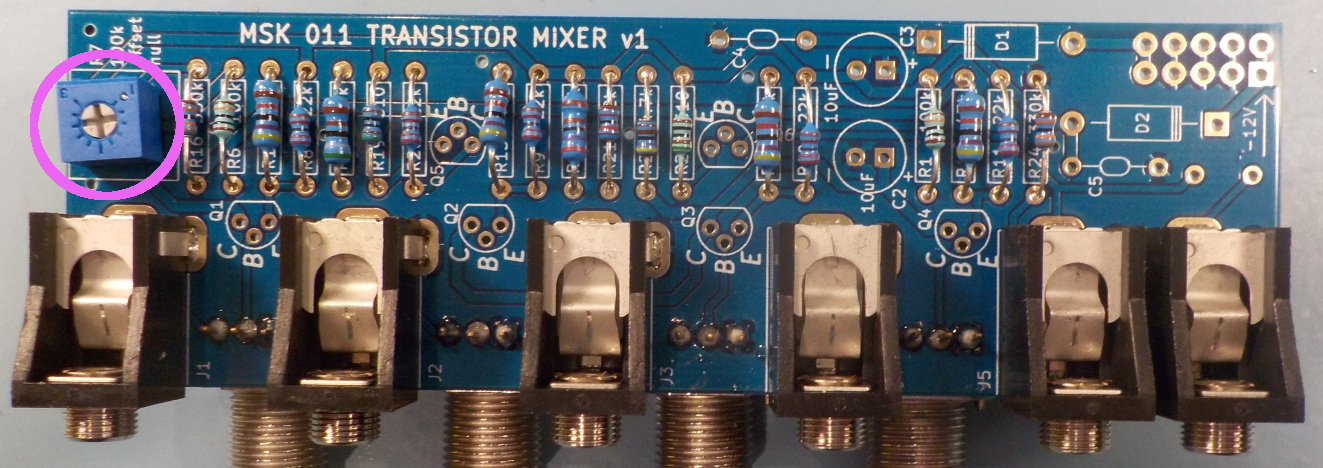
\includegraphics[width=\linewidth]{pot-100k.jpg}

\section{Transistors}

The six NPN transistors in this project are polarized and must be installed
in the correct orientation to work; that orientation is shown by the
silkscreen symbols.  Install each component so that its flat side points in
the same direction as the flat side shown on the silkscreen.  The three legs
of the component must be carefully bent into the same triangular pattern
(left and right forward, middle backward) as the holes on the board, and
then the component pressed into place.  There should be a gap of about three
millimetres between the board and the component body; do not attempt to seat
the component flush on the board because of the risk of breaking off the
legs where they enter the body.

To aid in modifications with different components, the three holes for each
transistor are also labelled with the letters ``E,'' ``B,'' and ``C,'' for
``emitter,'' ``base,'' and ``collector.''  If you are using some other
transistors, connect them to match those markings according to the pinout of
the parts you are using, even if that puts the flat side of the package other
than where it is shown on the silkscreen.

The solder pads for these components are smaller and closer together than
for any other through-hole components in the project, and the components
themselves tend to be relatively heat-sensitive.  Solder them carefully,
avoiding creating any solder bridges between adjacent pads.  Do not use
excessive time and heat trying to get the solder to flow through the board
and fillet on both sides, especially not on pads connected to the ground
plane; two-sided fillets may happen naturally, but it is enough for solder
to completely cover the pad on one side.

Install the six 2N5088 transistors Q1 to Q6.

\nopagebreak
\noindent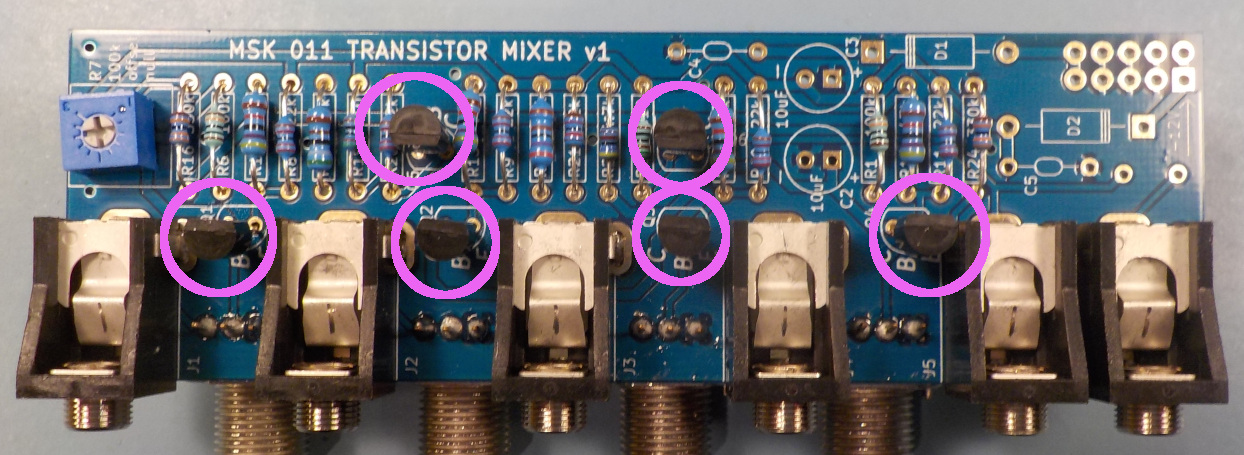
\includegraphics[width=\linewidth]{2n5088.jpg}

\section{Diodes}

Install the two Schottky diodes D1 and D2.  These protect the module against
reverse connection of the power supply.  They are polarized and must be
installed in the correct direction; otherwise they will prevent the module
from operating.  One end of each diode will be marked, usually with a stripe
of grey paint around the black plastic body of the diode.  That end is
called the
\emph{cathode}.  The diode outline on the PCB silkscreen is marked with a
similar stripe showing the direction of the cathode, and the solder pad for
the cathode is square instead of round.

\nopagebreak
\noindent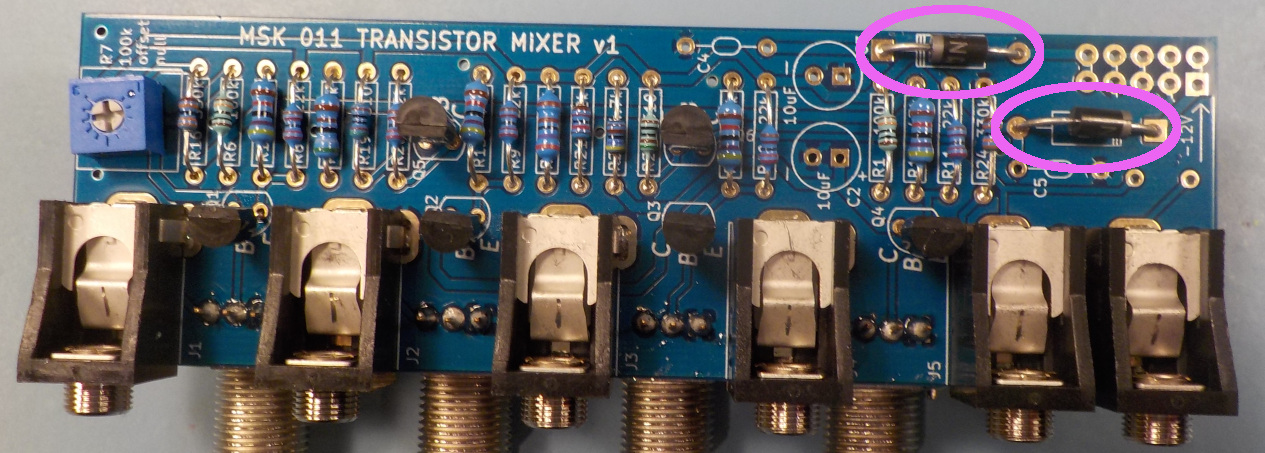
\includegraphics[width=\linewidth]{schottky.jpg}

\pagebreak

\section{Capacitors}

Install the two 0.1$\mu$F ceramic capacitors C4 and C5.  These filter out
high-frequency interference on the power supply lines.  These capacitors are
not polarized and may be installed in either orientation.

\nopagebreak
\noindent\includegraphics[width=\linewidth]{{cap-0.1u}.jpg}

Install the two 10$\mu$F electrolytic capacitors C2 and C3.  These filter
lower-frequency interference on the power lines.
They are polarized components, and may explode if connected
backwards.  As such, there are multiple clues to help you install them in
the right direction.  The negative leg of each capacitor will be marked in
some way, usually with a printed stripe and minus signs on the plastic
wrapping of the capacitor body.  The negative leg of the capacitor will
usually also be shorter, though that is less reliable than the body
markings.  On the PCB, the positive and negative pads are marked with
positive and negative signs in the silkscreen, and the solder pads
themselves are round for negative and square for positive.

\noindent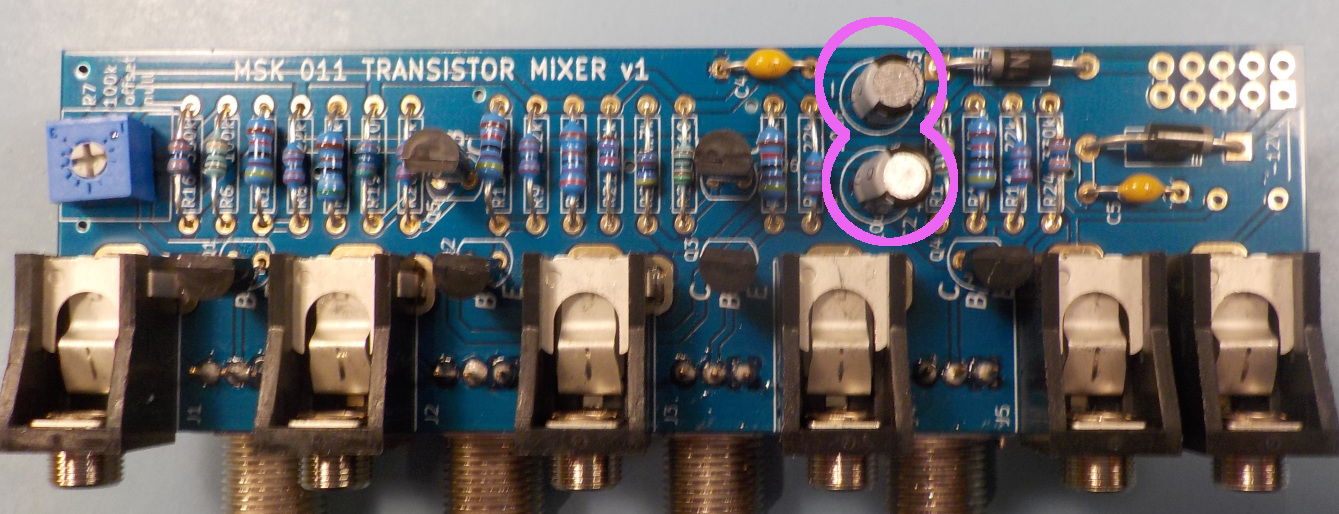
\includegraphics[width=\linewidth]{cap-10u.jpg}

Install the 4.7$\mu$F film capacitor C1.  This capacitor provides AC
coupling for the corresponding output.  It goes on the back of the board,
and needs to be installed at this point, late in the build, so as not to
conflict with the solder connections of other nearby components.  It is not
polarized and may be installed in either direction.

\noindent\includegraphics[width=\linewidth]{{cap-4.7u}.jpg}

\section{Power header}

Install the 10-pin dual-row Eurorack power header J7.  This header goes on
the back of the board, with C1 and the panel pots, opposite from most of the
other components.  It is not polarized
in the horizontal plane.  However, if it has shorter legs on one side, then
those are the ones that should go through the PCB (leaving the longer legs
sticking up to mate with the connector on the power cable), and if it has
tin plating on one end of the pins and gold on the other, then the tin side
should be the one soldered through the board.  Secure the header carefully
to the board, possibly with tape, before soldering it.  It is easy to
accidentally solder it at an angle, which is a difficult error to fix and
may cause trouble when you later attach the power cable.

\noindent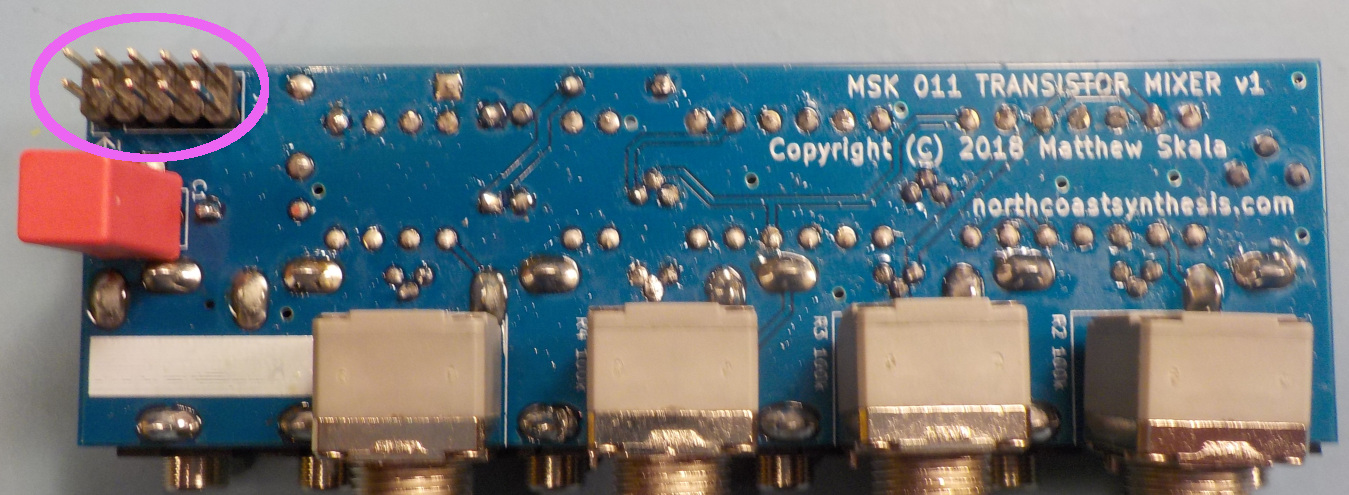
\includegraphics[width=\linewidth]{power.jpg}

Note that Eurorack power connections are polarized even if the connectors
are not.  The cables are usually grey ribbon type with a red stripe along
one side indicating pin 1, which carries $-$12V power.  For most modules
including the MSK~011, the red stripe should be at the \emph{bottom} when
the module is mounted vertically in a case.  On the MSK~011, the correct
location of the $-$12V supply is also marked with the text ``$-$12V'' and
arrows on both sides of the PCB silkscreen.  This module is also protected
(by the Schottky diodes you just installed) from damage in case of a
reversed power connection; if you connect the power backwards and nothing
else is wrong, then the module will not power up but will be fine once you
connect the power correctly.  However, many other modules are not so
protected, and it is dangerous to get into the habit of depending on
protection diodes.  Destroying a module by connecting power backwards is
almost a rite of passage for Eurorack users.

\section{Final assembly}

If you have removed the panel, reattach it; if you have left it in place,
undo the nuts on the potentiometers and add the rest of the hardware.
The sequence of hardware for the potentiometers is first (nearest
the panel) the conical spring washer, high side in the middle and low side
around the outside; then the toothed lock-washer; then the nut.
In the case of the jack sockets, the knurled nuts provided for these will
have screwdriver slots on one side, and those should face the outside with
the smoother side facing the panel.

Do not overtighten any of this hardware, and be careful, if you are
using wrenches or pliers, to avoid scratching the panel.  Wrapping the tool
jaws with tape may help.

Attach the knobs to the potentiometers.  Twist each shaft to its limits in
each direction to ascertain how the slot in the shaft corresponds to where
you want the knob pointer, then slide the knob onto the shaft in the correct
orientation and tighten the setscrew with a small flat screwdriver.

There is a rectangular white area on the back of the board
reserved for adding a serial number, signature, quality control marking, or
similar.  Use a fine-tipped permanent marker to write whatever you want
there.

Your module is complete.

\nopagebreak
\noindent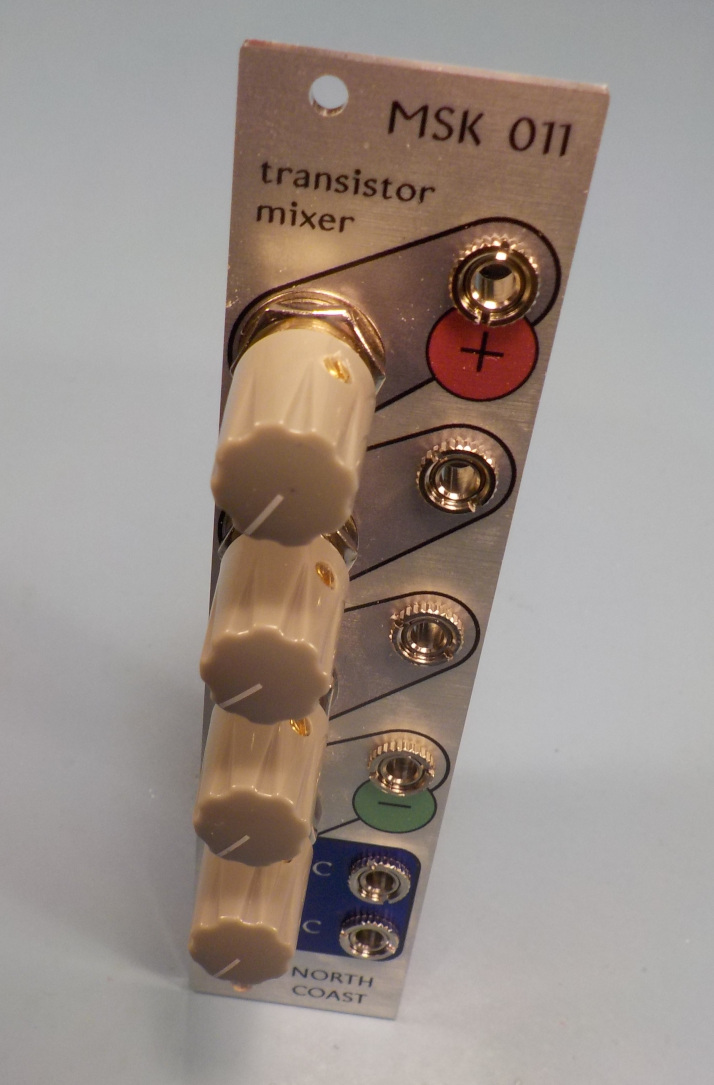
\includegraphics[width=\linewidth]{finished-module.jpg}
